%----------------------------------------------------------------------------------------
%	PACKAGES AND OTHER DOCUMENT CONFIGURATIONS
%----------------------------------------------------------------------------------------

\documentclass[DIV=calc, paper=a4, fontsize=12pt, twocolumn]{scrartcl}	 % A4 paper and 11pt font size

\usepackage{lipsum} % Used for inserting dummy 'Lorem ipsum' text into the template
\usepackage[utf8]{inputenc}
\usepackage[spanish,mexico]{babel}
\usepackage[protrusion=true,expansion=true]{microtype} % Better typography
\usepackage{graphicx}
\usepackage{amsmath,amsfonts,amsthm} % Math packages
\usepackage[svgnames]{xcolor} % Enabling colors by their 'svgnames'
\usepackage[hang, small,labelfont=bf,up,textfont=it,up]{caption} % Custom captions under/above floats in tables or figures
\usepackage{booktabs} % Horizontal rules in tables
\usepackage{fix-cm}	 % Custom font sizes - used for the initial letter in the document
\usepackage{xcolor}
\usepackage{sectsty} % Enables custom section titles
\allsectionsfont{\usefont{OT1}{phv}{b}{n}} % Change the font of all section commands
\definecolor{grisclaro}{RGB}{242, 242, 242}
\definecolor{rojo1}{RGB}{150, 0, 0}
\usepackage{fancyhdr} % Needed to define custom headers/footers
\pagestyle{fancy} % Enables the custom headers/footers
\usepackage{lastpage} % Used to determine the number of pages in the document (for "Page X of Total")

% Headers - all currently empty
\lhead{}
\chead{}
\rhead{}

% Footers
\lfoot{}
\cfoot{}
\rfoot{\footnotesize Page \thepage\ of \pageref{LastPage}} % "Page 1 of 2"

\renewcommand{\headrulewidth}{0.0pt} % No header rule
\renewcommand{\footrulewidth}{0.4pt} % Thin footer rule

\usepackage{lettrine} % Package to accentuate the first letter of the text
\newcommand{\initial}[1]{ % Defines the command and style for the first letter
\lettrine[lines=3,lhang=0.3,nindent=0em]{
\color{DarkGoldenrod}
{\textsf{#1}}}{}}

%----------------------------------------------------------------------------------------
%	TITLE SECTION
%----------------------------------------------------------------------------------------

\usepackage{titling} % Allows custom title configuration

\newcommand{\HorRule}{\color{DarkGoldenrod} \rule{\linewidth}{1pt}} % Defines the gold horizontal rule around the title

\pretitle{\vspace{-30pt} \begin{flushleft} \HorRule \fontsize{50}{50} \usefont{OT1}{phv}{b}{n} \color{DarkRed} \selectfont} % Horizontal rule before the title

\title{Actividad 1} % Your article title

\posttitle{\par\end{flushleft}\vskip 0.5em} % Whitespace under the title

\preauthor{\begin{flushleft}\large \lineskip 0.5em \usefont{OT1}{phv}{b}{sl} \color{DarkRed}} % Author font configuration

\author{Antonio Cota, } % Your name

\postauthor{\footnotesize \usefont{OT1}{phv}{m}{sl} \color{Black} % Configuration for the institution name
Universidad de Sonora % Your institution

\par\end{flushleft}\HorRule} % Horizontal rule after the title

\date{} % Add a date here if you would like one to appear underneath the title block

%----------------------------------------------------------------------------------------

\begin{document}

\maketitle % Print the title

\thispagestyle{fancy} % Enabling the custom headers/footers for the first page 

%----------------------------------------------------------------------------------------
%	ABSTRACT
%----------------------------------------------------------------------------------------

% The first character should be within \initial{}
\initial{E}\textbf{l análisis matemático de los péndulos en general es un poco complicado. Algunas suposiciones pueden ser hechas para simplificar, en el caso del péndulo simple permite que las ecuaciones de movimiento puedan ser resueltas analíticamente para oscilaciones pequeñas.}

%----------------------------------------------------------------------------------------
%	ARTICLE CONTENTS
%----------------------------------------------------------------------------------------

\section*{Péndulo simple}

EL llamado “péndulo simple” a una idealización del “péndulo real” pero en un sistema aislado se hacen las siguientes suposiciones:

\begin{itemize}
\item La barra o el cable en el cual la bola oscila es de masa despreciable, inextensible y siempre permanecerá tensa.
\item La bola es una masa puntual;
\item El movimiento ocurre solo en dos dimensiones, i.e. la bola puede no trazar una elipse pero si un arco.
\item El movimiento no pierde energía debido a la fricción o resistencia del aire.
\item El campo gravitacional es uniforme.
\item El soporte no es móvil.
\end{itemize}

La ecuación diferencial que representa el movimiento de un péndulo simple es 

\begin{equation}
\frac{d^{2}\theta}{dt^{2}} + \frac{g}{l}\sin{\theta} = 0
\end{equation}

La siguiente imagen es un ejemplo típico de un péndulo simple

\begin{figure}[hb]
  \centering
  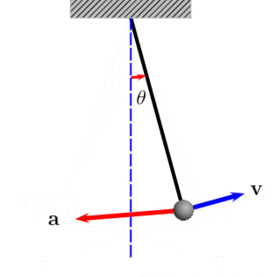
\includegraphics[width=2in]{pendulosimple}
  \caption[Close up of \textit{Hemidactylus} sp.]
   {Imagen de un péndulo simple mostrando los vectores velocidad y aceleración.}
\end{figure}

\begin{center}
{ \fboxsep 12pt
\fcolorbox {orange}{grisclaro}{
\begin{minipage}[t]{7.5cm}
\subsection*{Derivación de la ecuación (1) a partir del concepto “Fuerza”}
\vspace{0.5cm}
Considérese la Figura 2, en cual se muestra las fuerzas que actúan en un péndulo simple. Tenga en cuenta que la ruta del péndulo barre un arco de un círculo. El ángulo $\theta$ es medido en radianes, y esto es crucial para la ecuación (1). La flecha azul es la fuerza gravitacional que actúa en la bola, y la flecha violeta es la misma fuerza pero resuelta en su componente vertical y perpendicular al movimiento instantáneo de la bola. 

\end{minipage}
} }
\end{center}

\newpage

\begin{center}
{ \fboxsep 12pt
\fcolorbox {orange}{grisclaro}{
\begin{minipage}[t]{7.5cm}

La dirección de la velocidad instantánea perteneciente a la bola siempre apunta a lo largo del eje rojo, el cual es considerado el eje tangencial porque su dirección es siempre tangente al círculo.

\end{minipage}
} }
\end{center}

\vspace{0.05cm}

\begin{figure}[hb]
  \centering
  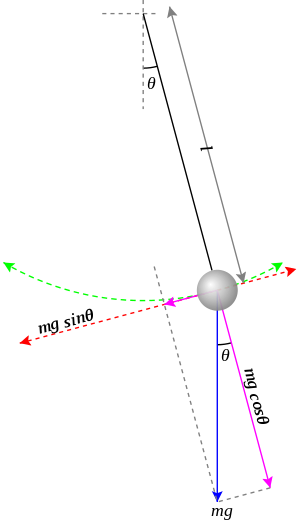
\includegraphics[width=2in]{pendulosimple2.png}
  \caption[Close up of \textit{Hemidactylus} sp.]
   {Diagrama de fuerzas para un péndulo \\ simple.}
\end{figure}

\begin{center}
{ \fboxsep 12pt
\fcolorbox {orange}{grisclaro}{
\begin{minipage}[t]{7.5cm}

Considére la segunda ley de Newton,

$$F=ma$$

donde $F$ es la suma de todas las fuerzas sobre el objeto, $m$ es masa, y $a$ es la aceleración. Debido a que sólo estamos tomando en cuenta los cambios en la velocidad, y ya que la bola esta forzada a moverse en un camino circular, aplicaremos la ecuación de Newton únicamente al eje tanqgencial. La pequeña flecha violeta representa la componente de la fuerza gravitacional que esta sobre el eje tangencial, podemos utilizar trigonometría para determinar su magnitud. Entonces,

$$F=-mg\sin{\theta}=ma$$
$$a=-g\sin{\theta}$$

\end{minipage}
} }
\end{center}

\vspace{0.5cm}

\begin{center}
{ \fboxsep 12pt
\fcolorbox {orange}{grisclaro}{
\begin{minipage}[t]{7.5cm}

donde $g$ es la aceleración debida a la gravedad cerca de la superficie de la tierra. El signo negativo que esta a lado derecho implica que $\theta$ y $a$ siempre apuntan en direcciones opuestas. Esto tiene sentido porque cuando el péndulo oscila hacia la izquierda, nosotros esperamos que se acelere hacia la derecha.\\

La aceleración lineal $a$ a lo largo del eje rojo puede ser relacionada con el cambio del ángulo $\theta$ con la fórmula de longitud de arco; $s$ es la longitud de arco

$$ s=l\theta$$
$$ v= \frac{ds}{dt} = l\frac{d\theta}{dt}$$
$$ a= \frac{d^{2}s}{dt^{2}} = l\frac{d^{2}\theta}{dt^{2}}$$
\vspace{0.5cm}
así:

$$ l\frac{d^{2}\theta}{dt^{2}} = -g\sin{\theta}$$
$$ \frac{d^{2}\theta}{dt^{2}} +\frac{g}{l}\sin{\theta} = 0 $$

\end{minipage}
} }
\end{center}

\vspace{0.3cm}
\begin{center}
{ \fboxsep 12pt
\fcolorbox {rojo1}{grisclaro}{
\begin{minipage}[t]{7.5cm}
\subsection*{Derivación de la ecuación (1) a partir del concepto “Torque”}
\vspace{0.5cm}
La ecuación (1) puede ser obtenida usando las dos definiciones para el torque.

$$ \tau = \boldsymbol{l} \times \boldsymbol{F} = \frac{d\boldsymbol{L}}{dt}$$

Empezaremos con la definición de torque para una bola en un péndulo usando la fuerza debida a la gravedad.

$$ \tau = \boldsymbol{l} \times \boldsymbol{F_{g}}$$

donde $\boldsymbol{l}$ es vector longitud del péndulo y $\boldsymbol{F_{g}}$ es la fuerza debida a la gravedad.\\

Por ahora solo consideremos la magnitud del torque sobre el péndulo.
\end{minipage}
} }
\end{center}

\newpage

\begin{center}
{ \fboxsep 12pt
\fcolorbox {rojo1}{grisclaro}{
\begin{minipage}[t]{7.5cm}

\providecommand{\abs}[1]{\lvert#1\rvert}
\providecommand{\norm}[1]{\lVert#1\rVert}

$$  \abs{\tau} = -mgl\sin{\theta} $$

donde $m$ es la masa del péndulo, $g$ es la aceleración debida a la gravedad, $l$ es la longitud del péndulo y $\theta$ es el ángulo entre el vector de longitud y la fuerza gravitacional.\\

Ahora reescribiremos el momento angular.

$$ \boldsymbol{L} = \boldsymbol{r} \times \boldsymbol{p} = m\boldsymbol{r} \times (\omega \times \boldsymbol{r})$$

Nuevamente solo consideremos la magnitud del momento angular.

$$ \abs{\boldsymbol{L}} = mr^{2}\omega = ml^{2}\frac{d\theta}{dt}$$

De acuerdo con $\tau = \frac{d\boldsymbol{L}}{dt}$, podemos obtenerla comparando sus magnitudes

$$-mgl\sin{\theta} = ml^{2}\frac{d^{2}\theta}{dt^{2}}$$

entonces:

$$ \frac{d^{2}\theta}{dt^{2}} +\frac{g}{l}\sin{\theta} = 0 $$

este es el mismo resultado que se obtuvo en el análisis de fuerzas.


\end{minipage}
} }
\end{center}

\begin{center}
{ \fboxsep 12pt
\fcolorbox {rojo1}{grisclaro}{
\begin{minipage}[t]{7.5cm}
\subsection*{Derivación de la ecuación (1) a partir del concepto “Energía”}
\vspace{0.5cm}
También puede ser obtenida mediante el principio de la conservación de la energía mecánica: cualquier objeto que cae desde una distancia vertical $h$ adquiriría energía cinética igual a la que perdería en la caída. En otras palabras, la energía potencial gravitacional es convertida a energía cinética. \\
El cambio en la energía potencial esta dada por

$$ \Delta U = mgh$$

el cambio en la energía cinética (el cuerpo empieza del reposo) esta dada por

\end{minipage}
} }
\end{center}

\begin{center}
{ \fboxsep 12pt
\fcolorbox {rojo1}{grisclaro}{
\begin{minipage}[t]{7.5cm}

$$ \Delta K = \frac{1}{2}mv^{2}$$

Dado que no se pierde energía, la ganancia en una debe ser igual a la perdida en la otra.

$$\frac{1}{2}mv^{2} = mgh$$

\end{minipage}
} }
\end{center}

\begin{figure}[hb]
  \centering
  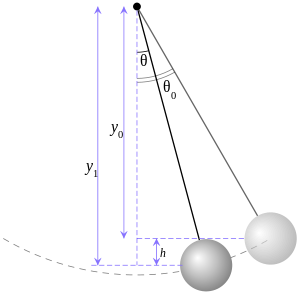
\includegraphics[width=2in]{pendulosimple3.png}
  \caption[Close up of \textit{Hemidactylus} sp.]
   {Trigonometría de un péndulo simple.}
\end{figure}

\begin{center}
{ \fboxsep 12pt
\fcolorbox {rojo1}{grisclaro}{
\begin{minipage}[t]{7.5cm}

El cambio en la velocidad en términos de la altura puede ser expresada como

$$ v = \sqrt{2gh}$$

Usando la fórmula para la longitud de arco de arriba, esta ecuación puede reescribirse en términos de $\frac{d\theta}{dt}$

$$ v = l\frac{d\theta}{dt} = \sqrt{2gh}$$
$$ \frac{d\theta}{dt} = \frac{1}{l}\sqrt{2gh}$$

$h$ es la distancia vertical desde donde el péndulo cae. Observar la Figura 3, represeta la trigonometría de un simple péndulo. Si el péndulo empieza a oscilar desde algún ángulo inicial $\theta_{0}$, luego $y_{0}$, la distancia vertical desde el soporte, está dada por

$$y_{0} = l\cos{\theta_{0}}$$

similarmente, para $y_{1}$, tenemos

$$y_{1} = l\cos{\theta}$$

\end{minipage}
} }
\end{center}

\begin{center}
{ \fboxsep 12pt
\fcolorbox {rojo1}{grisclaro}{
\begin{minipage}[t]{7.5cm}

así $h$ es la diferencia de esas dos últimas ecuaciones

$$ h = l(\cos{\theta} - \cos{\theta_{0}}$$

en términos de $\frac{d\theta}{dt}$ nos da

$$ \frac{d\theta}{dt} = \sqrt{\frac{2g}{l}(\cos{\theta} - \cos{\theta_{0}})}$$

Esta ecuación es conocida como la {\it{primera integral de movimiento}}, nos da la velocidad en terminos de la ubicación e incluye la constante de integración relacionada con el desplazamiento inicial $(\theta_{0})$. Podemos derivarla aplcando la regla de la cadena, con respecto al tiempo para obtener la aceleración

$$ \frac{d}{dt}\frac{d\theta}{dt} = \frac{d}{dt}\sqrt{\frac{2g}{l}(\cos{\theta} - \cos{\theta_{0}})}$$

$$\frac{d^{2}\theta}{dt^{2}} = \frac{1}{2}\frac{-(2g/l)\sin{\theta}}{\sqrt{(2g/l)(\cos{\theta}-\cos{\theta_{0}})}}\frac{d\theta}{dt} =$$

$$ {\small \frac{1}{2}\frac{-(2g/l)\sin{\theta}}{\sqrt{(2g/l)(\cos{\theta}-\cos{\theta_{0}})}}\sqrt{\frac{2g}{l}(\cos{\theta} - \cos{\theta_{0}})}}$$

$$ = -\frac{g}{l}\sin{\theta}$$

mismo resultado al de análisis de fuerzas.

\end{minipage}
} }
\end{center}

\vspace{0.5cm}

\section*{Aproximaciones a oscilaciones pequeñas}
\vspace{0.5cm}
La ecuación diferencial (1) no se puede resolver fácilmente, no hay solución que se puede escribir en términos de funciones elementales. Aún así podemos añadir una restricción al tamaño de la amplitud de oscilación y así nos da una solución que puede ser resuelta fácilmente. Si asumimos que el ángulo es mucho menor que 1 radián, o 

$$ \theta \ll 1 $$

\vspace{2cm}

entonces sustituimos para $\sin{\theta}$ en la ecuación (1) usando aproximaciones para ángulos pequeños,

$$\sin{\theta} \approx \theta $$

nos genera la ecuación de un oscilador armónico 

$$ \frac{d^{2}\theta}{dt^{2}} + \frac{g}{l}\theta = 0 $$

El error debido a la aproximación es del orden de $\theta^{3}$ (de la serie de Maclaurin para $\sin{\theta}$\\

Dadas las condiciones iniciales $\theta(0) = \theta_{0}$ y $d\theta/dt(0) = 0$, la solución resulta,

\begin{center}
{ \fboxsep 12pt
\fcolorbox {black}{white}{
\begin{minipage}[t]{7.5cm}

$$\theta(t) = \theta_{0}\cos{(\sqrt{\frac{g}{l}t})} \quad \quad \quad \theta_{0} \ll 1$$

\end{minipage}
} }
\end{center}

El movimiento es un simple movimiento armónico donde $\theta_{0}$ es la semi-amplitud de la oscilación (eso es, el ángulo máximo entre la barra y la vertical). El período de movimiento, el tiempo para una oscilación completa es 

\begin{center}
{ \fboxsep 12pt
\fcolorbox {black}{white}{
\begin{minipage}[t]{7.5cm}

$$T_{0} = 2\pi \sqrt{\frac{l}{g}} \quad \quad \quad \quad \quad \theta_{0} \ll 1 $$

\end{minipage}
} }
\end{center}

la cual es conocida como la ley de Christiaan Huygen's para el período. Notar que para oscilaciones pequeñas, el período es independiente de la amplitud $\theta_{0}$; esa es la propiedad de isocronismo que Galileo descubrió.

\vspace{0.5cm}

\subsection*{Regla de oro para la longitud del péndulo}

$$ T_{0} = 2\pi \sqrt{\frac{l}{g}} $$

puede ser expresada como

$$ l = \frac{g}{\pi^{2}} \times \frac{T_{0}^{2}}{4}$$

\newpage

Si son utilizadas las unidades del SI (i.e. mediciones en metros y segundos), y asumiendo que las mediciones toman lugar en la superficie de la tierra, entonces $g \approx 9.81 \quad m/s^{2}$ y $g/\pi^{2} \approx 1$ (0.994 es la aproximación para 3 decimales).\\

Por lo tanto, una aproximación relativa razonable para la longitud y el período son,

$$l \approx \frac{T_{0}^{2}}{4}$$
$$T_{0} \approx 2\sqrt{l}$$

donde $T_{0}$ son los segundos entre dos pulsos (un pulso por cada lado de la oscilación), y $l$ es medido en metros.

\subsection*{Período para amplitudes aribitarias}
\vspace{0.5cm}

Para amplitudes más allá de la aproximación para ángulos pequeños, se puede computar el período exacto si primero se invierte la ecuación paa la velocidad angular obtenida desde el método de la energía,

$$ \frac{dt}{d\theta} = \sqrt{\frac{l}{2g}}\frac{1}{\sqrt{\cos{\theta}-\cos{\theta_{0}}}}$$

después integrando sobre un ciclo completo

$$ T = t(\theta_{0} \rightarrow 0 \rightarrow -\theta_{0} \rightarrow 0 \rightarrow \theta_{0})$$

o dos veces un medio ciclo

$$T= 2t(\theta_{0} \rightarrow 0 \rightarrow -\theta_{0})$$

o 4 veces un cuarto de ciclo

$$T = 4t(\theta_{0} \rightarrow 0)$$

lo que nos da

$$ T = 4\sqrt{\frac{l}{2g}}\int_{0}^{\theta_{0}}\frac{1}{\sqrt{\cos{\theta}-\cos{\theta_{0}}}}d\theta$$.

Notar que esta integral diverge como $\theta_{0}$ se aproxima a la vertical

$$\lim_{\theta_{0} \to \pi}{T} = \infty$$

de manera que un péndulo aún con la energía suficiente nunca llegará a la vertical. (a la inversa, un péndulo cerca del máximo le tomará un largo tiempo para que descienda.)

\begin{figure}[hb]
  \centering
  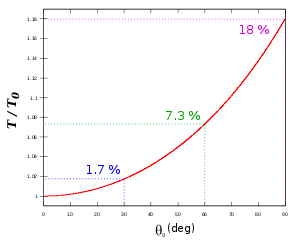
\includegraphics[width=2in]{pendulosimple4.png}
  \caption[Close up of \textit{Hemidactylus} sp.]
   {La desviación de un período “verdadero” para un péndulo desde una aproximación de oscilaciones pequeñas. }
\end{figure}
\vspace{0.5cm}

La integral puede ser reescrita en términos de integrales elípticas como

$$ T= 4\sqrt{\frac{l}{g}}F(\frac{\theta_{0}}{2},\csc{\frac{\theta_{0}}{2}})\csc{\frac{\theta_{0}}{2}}$$

donde $F$ es la integral elíptica incompleta de primer tipo definida como

$$F(\phi,k) = \int_{0}^{\phi}\frac{1}{\sqrt{1-k^{2}\sin^{2}{u}}}du$$

o más concisa con la sustitución de $\sin{u} = \frac{\sin{\frac{\theta}{2}}}{\sin{\frac{\theta_{0}}{2}}}$ expresando $\theta$ en términos de $u$,

\begin{equation}
T = 4\sqrt{\frac{l}{g}}K(\sin^{2}{\frac{\theta_{0}}{2}})
\end{equation}


donde $K$ es la integral elíptica completa de primer tipo definida como 

$$ K(k) = F(\frac{\pi}{2},k)$$
$$ = \int_{0}^{\pi/2}\frac{1}{\sqrt{1-k^{2}\sin^{2}{u}}}du$$ 

Para una comparación a la aproximación de la solución completa, consideremos el período de un péndulo de longitud 1 m en la tierra ($g=9.80665 \quad m/s^{2}$) un ángulo inicial de 10 grados es $4\sqrt{\frac{1m}{g}}K(\sin^{2}{(\frac{10^{\circ}}{2})} \approx 2.0102 s.$

La aproximación lineal nos da $2\pi\sqrt{\frac{1m}{g}} \approx 2.0064s.$

La diferencia entre estos dos valores, es menor que el 0.2\% es mucho menor que la causada por la variación de $g$ .

Desde aquí hay muchas maneras de calcular la integral elíptica:

\begin{figure}[hb]
  \centering
  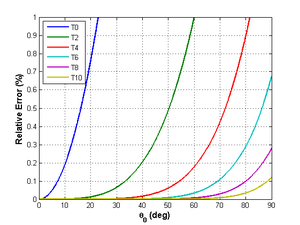
\includegraphics[width=2in]{pendulosimple5.png}
  \caption[Close up of \textit{Hemidactylus} sp.]
   {Errores relativos utilizando la serie de potencias. }
\end{figure}
\vspace{0.5cm}


\subsection*{Polinomios de Legendre para la solución de la integral elíptica}
\vspace{0.5cm}

Con la ecuación (2) y los polinomios de Legendre para la solución de la integral elíptica tenemos:

$$K(k)=\frac{\pi}{2}\{ 1 + (\frac{1}{2})^{2}k^{2} + (\frac{1\cdot 3}{2\cdot 4})^{2}k^{4} + \ldots + $$
$$+ [\frac{(2n-1)!!}{(2n)!!}]^{2}k^{2n} + \ldots \} $$

donde $n!!$ denota el doble factorial, una solución exacta para el período del péndulo es:

$$T=2\pi\sqrt{\frac{l}{g}}(1 + (\frac{1}{2})^{2}\sin^{2}{\frac{\theta_{0}}{2}} + (\frac{1\cdot3}{2\cdot4})^{2}\sin^{4}{\frac{\theta_{0}}{2}}+ $$

$$+ (\frac{1\cdot3\cdot5}{2\cdot4\cdot6})^{2}\sin^{6}{\frac{\theta_{0}}{2}}+ \ldots)$$

$$T=2\pi\sqrt{\frac{l}{g}}\cdot\sum_{n=0}^{\infty}[(\frac{(2n)!}{(2^{n}\cdot n!)^{2}})^{2}\cdot \sin^{2n}{(\frac{\theta_{0}}{2})}]$$

La Figura 5 muestra los errores relativos usando las series de potencias. $T_{0}$ es la aproximación lineal, y $T_{2}$ hasta $T_{10}$ incluye los términos respectivos para las potencias desde la segunda hasta la décima potencia.

\subsection*{Soluciones en series de potencias para la integral elíptica}
\vspace{0.5cm}

Otra formulación para la solución de arriba puede ser obtenida usando las series de Maclaurin:

$$ \sin{\frac{\theta_{0}}{2}} = \frac{1}{2}\theta_{0} - \frac{1}{48}\theta_{0}^{3} + \frac{1}{3840}\theta_{0}^{5} - \frac{1}{645120}\theta_{0}^{7} + \ldots $$

es usada en la solución de arriba en términos de polinomios de Legendre. La serie de potencia resultante es:

$$T=2\pi\sqrt{\frac{l}{g}}(1+\frac{1}{16}\theta_{0}^{2} + \frac{11}{3072}\theta_{0}^{4} + \frac{173}{737280}\theta_{0}^{6}+$$

$$ + \frac{22931}{1321205760}\theta_{0}^{8} + \frac{1319183}{951268147200}\theta_{0}^{10} + \ldots )$$

\begin{figure}[hb]
  \centering
  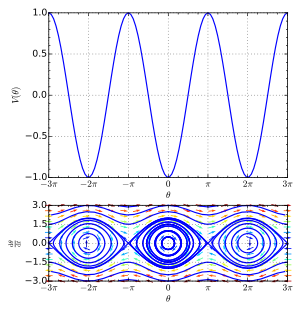
\includegraphics[width=2in]{pendulosimple6.png}
  \caption[Close up of \textit{Hemidactylus} sp.]
   {Energía potencial y retrato de fase de un péndulo simple. Tenga en cuenta que el eje x, siendo el ángulo, se envuelve sobre sí mismo después de cada $2\pi$ radianes}
\end{figure}
\vspace{0.5cm}

\subsection*{Media aritmética-geométrica de la solución para la integral elíptica}
\vspace{0.5cm}

De la ecuación (2) y la media aritmética-geométric para la integral elíptica:

$$K(k) = \frac{\pi/2}{M(1-k,1+k)}$$

donde $M(x,y)$ es la media aritmética-geométrica para $x$ y $y$. Esto nos da una fórmula alternativa que converge rápidamente al período:

$$ T = \frac{2\pi}{M(1,\cos{\frac{\theta_{0}}{2}})}\sqrt{\frac{l}{g}}$$

%----------------------------------------------------------------------------------------
%	REFERENCE LIST
%----------------------------------------------------------------------------------------

\begin{thebibliography}{99} % Bibliography - this is intentionally simple in this template



\bibitem[Nelson, Robert; M. G. Olsson]{February 1986}
\newblock "The pendulum — Rich physics from a simple system".
\newblock American Journal of Physics 54 (2): pp. 112–121. doi:10.1119/1.14703. Retrieved 2012-04-30.

\bibitem[Carvalhaes, Claudio G.; Suppes, Patrick]{December 2008}
\newblock "Approximations for the period of the simple pendulum based on the arithmetic-geometric mean".
\newblock  Am. J. Phys. 76 (12): 1150–1154, doi:10.1119/1.2968864, ISSN 0002-9505, retrieved 2013-12-14

\bibitem[Adlaj, Semjon]{September 2012}
\newblock "An eloquent formula for the perimeter of an ellipse".
\newblock  Notices of the AMS 76 (8): 1094–99, doi:10.1090/noti879, ISSN 1088-9477

\bibitem[ Van Baak, Tom]{November 2013}
\newblock "A New and Wonderful Pendulum Period Equation".
\newblock  Horological Science Newsletter 2013 (5): 22–30.

\end{thebibliography}

%----------------------------------------------------------------------------------------

\end{document}